\chapter{System Evaluation of Testing Application}
\label{cha:evaluation}

This chapter evaluates the \textit{Guardians of the Chess Grandmaster} web application against the objectives established in ~\textit{Chapter} \ref{cha:introduction}. It presents the results of automated testing across the \texttt{frontend} and \texttt{backend}, discusses the deployment of the system to cloud platforms, assesses how well the implemented system meets its functional objectives, and reflects critically on the limitations of the approach and opportunities for future improvement.

\section{Testing the Application}
\label{sec:testing}

A comprehensive suite of automated tests was written to verify the correctness and robustness of the system. Testing was divided into two primary concerns: the \texttt{frontend} React application and the \texttt{backend} Node.js/Express.js API. The pages and components tested cover the full surface area of the application, spanning the following major views:

\begin{itemize}
    \item \textbf{Landing} $\rightarrow$ unauthenticated entry point and sign-in flow
    \item \textbf{Home} $\rightarrow$ authenticated dashboard and navigation hub
    \item \textbf{Play} $\rightarrow$ chess game interface including board, timer, and move history
    \item \textbf{Tutorial} $\rightarrow$ interactive chess learning content
    \item \textbf{Friends} $\rightarrow$ social features including friend requests, challenges, and chat
    \item \textbf{Profile} $\rightarrow$ user statistics and game history
    \item \textbf{Settings} $\rightarrow$ account and preference management
\end{itemize}

\subsection*{Frontend Testing}

The \texttt{frontend} was built using \textbf{React} with \textbf{TypeScript}, and all component and page tests were written using the \textbf{Jest} testing framework together with \textbf{React Testing Library}. Tests were executed by running the following command from the project root \texttt{cd frontend \&\& npm run test}.

As shown in Figure~\ref{fig:testF}, the test runner reported \textbf{39 test files} and \textbf{132 individual tests}, all of which passed. Tests were organised across two top-level directories: \texttt{Components/} and \texttt{Pages/}.

\begin{figure}[ht]
    \centering
    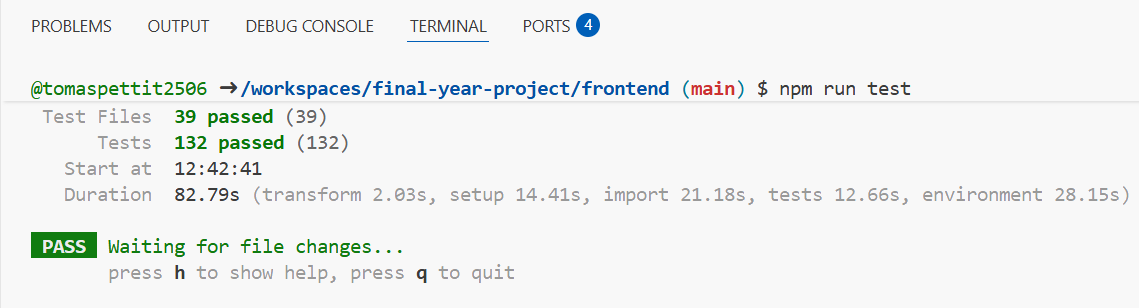
\includegraphics[width=0.85\linewidth]{images/Evaluation_Image/Testing_Frontend.png}
    \caption{Frontend Automated Test Results}
    \label{fig:testF}
\end{figure}

\subsubsection*{Component Tests}

The \texttt{Components/} directory was subdivided into three feature-specific folders, each tested independently.

\subsubsection*{Page Tests}

In addition to component-level tests, each of the seven application pages was tested independently to verify that routing, rendering, and top-level behaviour operated correctly.

\subsubsection*{Discussion of Frontend Results}

The 100\% pass rate across all 132 \texttt{frontend} tests demonstrates that the React components and pages render correctly, respond to user interactions as expected, and handle edge cases including empty states and loading conditions. The breadth of coverage — spanning the chess board, game controls, timer, move history, promotion dialogs, tutorial content, friend management, and PWA installation prompt — provides strong confidence in the structural correctness of the UI layer. That said, the tests are primarily unit and shallow-render tests; they confirm that components behave as specified in isolation but do not verify real browser interactions end-to-end. Full end-to-end testing using a tool such as \textbf{Cypress} or \textbf{Playwright} would provide additional assurance that complete user journeys function correctly in a deployed environment.

\subsection*{Backend Testing}

The \texttt{backend} was implemented using \textbf{Node.js} with the \textbf{Express.js} framework, with \textbf{Jest} used as the test runner for \texttt{backend} tests as well. Tests were executed using the following terminal command \texttt{cd backend \&\& npm run test}

As shown in Figure~\ref{fig:testB}, the test runner reported \textbf{9 test suites passed (9 total)} and \textbf{116 tests passed (116 total)}, with zero failures. This confirms that the \texttt{backend} API routes, middleware, and supporting logic behave correctly across all tested scenarios.

\begin{figure}[ht]
    \centering
    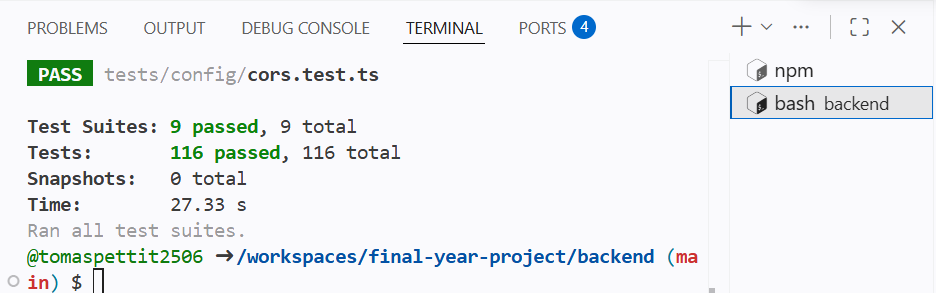
\includegraphics[width=0.9\linewidth]{images/Evaluation_Image/Testing_Backend.png}
    \caption{Backend Automated Testing Results}
    \label{fig:testB}
\end{figure}

\subsubsection*{Route Tests}

The \texttt{backend} test suite is organised under a \texttt{tests/routes/} directory, with one test file per route module. Table~\ref{table:testRoutes} presents the results for each route.

\begin{table}[ht]
    \centering
    \newcolumntype{s}{>{\columncolor[HTML]{AAACED}} l}
    \newcolumntype{t}{>{\columncolor[HTML]{FFFFFF}} l}
    \begin{tabular}{|s|t|}
        \hline
        \multicolumn{2}{|c|}{\cellcolor{green!15}Testing \texttt{tests/routes/}} \\
        \hline
        \textbf{Test File} & \textbf{Result} \\
        \hline
        \texttt{friends.test.ts}     & \cellcolor{green!25}PASS \\ \hline
        \texttt{gameInvites.test.ts} & \cellcolor{green!25}PASS \\ \hline
        \texttt{games.test.ts}       & \cellcolor{green!25}PASS \\ \hline
        \texttt{requests.test.ts}    & \cellcolor{green!25}PASS \\ \hline
        \texttt{users.test.ts}       & \cellcolor{green!25}PASS \\ \hline
    \end{tabular}
    \caption{Test results for \texttt{tests/routes/}}
    \label{table:testRoutes}
\end{table}

\subsubsection*{Discussion of Backend Results}

All five route modules — users, friends, requests, games, and game invites — passed their full test suites. This confirms that the REST API endpoints respond correctly to both valid and invalid inputs, that authentication middleware behaves as expected, and that CORS configuration permits the \texttt{frontend} to communicate with the \texttt{backend} without errors. The passing of \texttt{games.test.ts} and \texttt{gameInvites.test.ts} in particular provides evidence that the core game lifecycle — creation, invitation, acceptance, and completion — is handled reliably at the API level. As with the \texttt{frontend}, however, the \texttt{backend} tests focus on unit and route-level behaviour. Broader integration tests that exercise the interaction between multiple routes and services in sequence, as well as stress tests under concurrent load, would strengthen confidence in the system's behaviour under real-world conditions.

\subsection*{Deployment Testing}

Beyond automated tests, the system was validated in a deployed, production-like environment by hosting the \texttt{frontend} and \texttt{backend} on separate cloud platforms.

\subsubsection*{Frontend Deployment — Vercel}

The React \texttt{frontend} was deployed to \textbf{Vercel}, a platform optimised for modern JavaScript frameworks. Vercel's continuous deployment pipeline was connected to the GitHub repository, allowing every push to the main branch to trigger an automatic rebuild and redeployment. The deployment was verified by navigating to the live URL and confirming that all seven pages loaded correctly, that routing between pages functioned as expected, and that the application prompted users to install it as a Progressive Web App (PWA) on supported devices. Environment variables such as the \texttt{backend} API URL and any third-party service keys were configured securely through Vercel's project settings, keeping sensitive values out of the repository.

\subsubsection*{Backend Deployment — Railway}

The Node.js/Express.js \texttt{backend} was deployed to \textbf{Railway}, a cloud platform well-suited to persistent server workloads. Railway was configured to pull from the \texttt{backend} directory of the GitHub repository and to inject the required environment variables — including database connection strings and authentication secrets — at runtime. The deployment was verified by issuing HTTP requests to each of the API routes from the deployed \texttt{frontend}, confirming that user registration, login, friend management, and game creation all operated correctly in the cloud environment. The database, also provisioned through Railway, maintained persistent state across requests as expected.

\section*{Evaluation Against Functional Objectives}

This section assesses the degree to which the implemented system meets the functional objectives set out in the Introduction. The objectives are evaluated on the basis of the testing results presented above and \textbf{direct observation} of the deployed application.

\subsection*{Chess Gameplay Against a Grandmaster Engine}

A central objective of the project was to allow users to play chess against an engine that \textbf{emulates} grandmaster-level thinking, with the aim of challenging and training players to think more deeply about their moves. This was achieved through integration with \textbf{Stockfish}, one of the world's strongest open-source chess engines. The \texttt{ChessBoard}, \texttt{GameController}, and \texttt{GameScreen} components — all of which passed their automated tests — collectively implement the full game loop: move validation, engine response, position evaluation, and game termination. The timer component ensures that timed game formats are supported, adding competitive pressure consistent with real tournament conditions.

\subsection*{Move Accuracy Tracking and Feedback}

A key training objective was to provide players with feedback on the quality of their moves, rather than simply recording wins and losses. This was addressed through the \texttt{AccuracyStats} component, which passed its automated test and is responsible for computing and displaying move accuracy scores. By comparing the player's chosen move against the engine's preferred continuation at each step, the system quantifies how closely the player is thinking like a grandmaster. This feature directly supports the educational purpose of the platform.

\subsection*{Social and Multiplayer Features}

The project aimed to create a platform rather than a standalone tool, which required social features enabling users to connect, challenge, and play against one another. The Friends subsystem — comprising \texttt{AddFriends}, \texttt{FriendsList}, \texttt{PendingRequests}, \texttt{SentRequests}, \texttt{ChallengeDialog}, \texttt{GameInvites}, \texttt{GameDialog}, \texttt{ChatDialog}, and \texttt{ProfileDialog} — represents a substantial portion of the application and passed all of its tests. The corresponding \texttt{backend} routes (\texttt{friends.test.ts}, \texttt{requests.test.ts}, \texttt{gameInvites.test.ts}) also passed in full, confirming that the social graph and invitation system operate correctly end-to-end.

\subsection*{Tutorial and Learning Content}

To cater for players who are new to chess or who wish to consolidate their understanding of the rules and piece movements, a dedicated \texttt{Tutorial} section was implemented. \textbf{All eight} tutorial component tests passed, covering basic rules, individual piece guides, drawing conditions, and winning conditions. This provides evidence that the learning content is rendered correctly and that the interactive mini-board used for illustration is functional.

\subsection*{User Profiles and Progress Tracking}

The system maintains persistent user profiles, storing game history and statistics that allow players to track their improvement over time. The \texttt{Profile} page and associated \texttt{backend} \texttt{users} route both passed their respective tests, and the deployment to Railway confirmed that data persists correctly across sessions in the cloud-hosted database.

\subsection*{Progressive Web App (PWA) Support}

An additional objective was to make the application installable on mobile devices via PWA support, broadening accessibility beyond desktop browsers. The \texttt{InstallPWA} component passed its test, and the deployment to Vercel confirmed that the PWA manifest and service worker were served correctly, enabling installation on both Android and iOS devices.


\section{Limitations and Opportunities for Future Work}

Identifying limitations is not a sign of weakness — it is evidence of critical insight into the decisions made throughout the project. The following reflects honestly on areas where the system falls short of an ideal implementation and where future iterations could improve upon the current work.

\subsection*{Absence of End-to-End Tests}

The most significant gap in the current test strategy is the lack of end-to-end (E2E) tests. While the 132 \texttt{frontend} and 116 \texttt{backend} tests provide strong coverage at the unit and route level, they do not exercise complete user journeys — for example, a user registering, navigating to the Play page, completing a game against the engine, and reviewing their accuracy score. A tool such as \textbf{Cypress} or \textbf{Playwright} would enable this level of testing and would catch integration failures that unit tests cannot detect. This is a concrete and high-value area for future improvement.

\subsection*{Stockfish Integration Constraints}

The current integration with Stockfish runs the engine at a fixed or lightly configurable difficulty level. A more sophisticated implementation would expose graduated difficulty settings that more meaningfully adapt to the player's current skill level, providing a progressive challenge curve. Additionally, the depth and time budget allocated to Stockfish's search may create perceptible latency on slower devices or network conditions; optimising this — for example by running the engine in a Web Worker on the client side — would improve the responsiveness of the gameplay experience.

\subsection*{Limited Real-Time Infrastructure}

Real-time features such as live game challenges, in-game chat, and opponent move updates are implemented using periodic polling or basic event handling. A more scalable and responsive architecture would use \textbf{WebSockets} (e.g. via \textbf{Socket.IO}) to push updates to clients instantly rather than relying on polling intervals. This is particularly relevant for the multiplayer game invitation flow, where delays in receiving a challenge notification could degrade the user experience.

\subsection*{Database Scalability}

The current database schema and query patterns were designed for a small number of concurrent users typical of a final-year project. Under significant concurrent load — many simultaneous games, friend requests, and chat messages — query performance may degrade without indexing strategies and connection pooling tuned for scale. Future work could include load testing with a tool such as \textbf{k6} or \textbf{Artillery} to identify bottlenecks and implement appropriate optimisations.

\subsection*{Accessibility}

Chess interfaces present non-trivial accessibility challenges: a visual board with interactive pieces is inherently difficult to make screen-reader-friendly. The current implementation does not include a dedicated accessibility mode (such as a text-based board representation or keyboard-navigable move input). Addressing this in a future iteration would broaden the potential user base and align the application with \textbf{WCAG 2.1} guidelines.

\subsection*{Grandmaster Move Database}

The application's name and concept — \textit{Guardians of the Chess Grandmaster} — implies a comparison between the player's moves and those made by real grandmasters in historical games. An opportunity for future work would be to integrate an opening book or a database of annotated grandmaster games (such as those available from \textbf{Lichess} or \textbf{Chess.com} APIs), allowing the system to contextualise the player's decisions within the broader canon of expert play rather than relying solely on engine evaluation.


\section*{Summary}
\label{sec:eval-summary}

This chapter has demonstrated that the \textit{Guardians of the Chess Grandmaster} system is robust and functionally complete with respect to its core objectives. All 248 automated tests (132 \texttt{frontend}, 116 \texttt{backend}) passed, and the application was successfully deployed to production-grade cloud infrastructure on Vercel and Railway. The system delivers chess gameplay against a Stockfish engine, move accuracy feedback, social and multiplayer features, a structured tutorial, persistent user profiles, and PWA support — fulfilling each of the functional objectives set out at the outset of the project. The limitations identified — notably the absence of end-to-end tests, real-time WebSocket infrastructure, and an accessibility mode — provide a clear roadmap for a next iteration of the platform.